% !TeX program = xelatex
% =====================================================================
%  巴塞尔问题三解 —— 一篇含数学公式的 LaTeX 短文示例
%  编译方式：见同目录下的 build.ps1
%            powershell -ExecutionPolicy Bypass -File .\build.ps1
% =====================================================================
\documentclass[11pt,a4paper]{ctexart}

\usepackage[margin=2.4cm]{geometry}
\usepackage{amsmath,amssymb,amsthm,bm}
\usepackage{graphicx}
\usepackage{booktabs}
\usepackage{array}
\usepackage{float}
\usepackage{xcolor}
\usepackage{tikz}
\usepackage[colorlinks=true,
            linkcolor=blue!55!black,
            citecolor=blue!55!black,
            urlcolor=blue!55!black]{hyperref}

% ------------------------- 版式细节 -------------------------
\linespread{1.18}
\setlength{\parskip}{0.25em}
\allowdisplaybreaks

% 页眉默认会把节标题转成全大写，这里改回原样（保留中文与 Euler 的大小写）
\renewcommand{\sectionmark}[1]{\markboth{}{\thesection\quad #1}}

% ------------------------- 定理环境 -------------------------
\newtheorem{theorem}{定理}[section]
\newtheorem{lemma}[theorem]{引理}
\newtheorem{proposition}[theorem]{命题}
\newtheorem{corollary}[theorem]{推论}

\theoremstyle{definition}
\newtheorem{definition}[theorem]{定义}
\newtheorem{example}[theorem]{例}

\theoremstyle{remark}
\newtheorem*{remark}{注}

% ------------------------- 自定义命令 -------------------------
\newcommand{\dd}{\,\mathrm{d}}
\newcommand{\R}{\mathbb{R}}
\newcommand{\Z}{\mathbb{Z}}
\newcommand{\N}{\mathbb{N}}
\newcommand{\abs}[1]{\left\lvert #1 \right\rvert}
\newcommand{\norm}[1]{\left\lVert #1 \right\rVert}

% 用于突出显示核心结论的方框
\newcommand{\keybox}[1]{%
  \begin{center}%
    \fcolorbox{blue!45!black}{blue!4}{%
      \parbox{0.86\textwidth}{\centering\vspace{2pt}#1\vspace{2pt}}}%
  \end{center}%
}

\title{\bfseries 巴塞尔问题三解\\[6pt]
       \large 从 Fourier 级数、双重积分到 Euler 乘积}
\author{AI4Math 作业示例}
\date{\today}

\begin{document}

\maketitle
\thispagestyle{empty}

\begin{abstract}
\noindent
1735 年，Euler 算出了全体自然数平方倒数之和 $\sum_{n\ge 1} n^{-2}=\pi^{2}/6$，
终结了悬置九十年的 Basel 问题。本文用三条彼此独立的路径重新抵达这一结果：
Fourier 级数的逐点收敛、二重积分的变量替换，以及 Euler 的正弦无穷乘积。
三条路径所用的工具各不相同，却都指向同一个常数，这恰好展示了分析学中
``同一事实的多种证明''所特有的美感。文中所有公式均给出完整推导。
\end{abstract}

\tableofcontents
\vspace{1em}

% =====================================================================
\section{问题的提出}
% =====================================================================

Riemann $\zeta$ 函数在 $\Re(s)>1$ 上由 Dirichlet 级数定义：
\begin{equation}
  \zeta(s) \;=\; \sum_{n=1}^{\infty} \frac{1}{n^{s}},
  \qquad \Re(s) > 1 .
  \label{eq:zeta-def}
\end{equation}
取 $s=2$ 便得到本文的主角：
\begin{equation}
  \zeta(2) \;=\; \sum_{n=1}^{\infty}\frac{1}{n^{2}}
  \;=\; 1+\frac{1}{4}+\frac{1}{9}+\frac{1}{16}+\cdots
  \;\approx\; 1.6449340668\ldots
  \label{eq:zeta2}
\end{equation}

这个级数收敛得很慢：前 $10^{3}$ 项之和仅为 $1.6439$，前 $10^{6}$ 项也才到
$1.644933$。仅凭数值累加，几乎不可能猜出它的精确值。然而 Euler 发现
\begin{equation}
  \boxed{\;\zeta(2)=\frac{\pi^{2}}{6}\;}
  \label{eq:basel}
\end{equation}
下面我们给出三种证明。

% =====================================================================
\section{解法一：Fourier 级数}
% =====================================================================

\subsection{一个周期函数的展开}

考虑 $2\pi$-周期函数 $f(x)=x^{2}$ 在区间 $[-\pi,\pi]$ 上的限制。
它连续、分段 $C^{1}$，故其 Fourier 级数在每一点收敛到 $f$ 本身。
设
\begin{equation}
  f(x) \;\sim\; \frac{a_{0}}{2}+\sum_{n=1}^{\infty}
  \bigl(a_{n}\cos nx + b_{n}\sin nx\bigr),
\end{equation}
其中
\begin{equation}
  a_{n}=\frac{1}{\pi}\int_{-\pi}^{\pi} x^{2}\cos nx\dd x,
  \qquad
  b_{n}=\frac{1}{\pi}\int_{-\pi}^{\pi} x^{2}\sin nx\dd x .
\end{equation}
由于 $x^{2}\sin nx$ 是奇函数，$b_{n}=0$。对 $a_{n}$（$n\ge 1$）分部积分两次：
\begin{align}
  a_{n}
  &=\frac{1}{\pi}\left[\frac{x^{2}\sin nx}{n}\right]_{-\pi}^{\pi}
    -\frac{2}{n\pi}\int_{-\pi}^{\pi} x\sin nx\dd x \notag\\
  &=-\frac{2}{n\pi}\left(\left[-\frac{x\cos nx}{n}\right]_{-\pi}^{\pi}
    +\frac{1}{n}\int_{-\pi}^{\pi}\cos nx\dd x\right) \notag\\
  &=-\frac{2}{n\pi}\cdot\left(-\frac{2\pi\cos n\pi}{n}\right)
    =\frac{4(-1)^{n}}{n^{2}} .
  \label{eq:an}
\end{align}
而
\begin{equation}
  \frac{a_{0}}{2}=\frac{1}{2\pi}\int_{-\pi}^{\pi}x^{2}\dd x
  =\frac{1}{2\pi}\cdot\frac{2\pi^{3}}{3}=\frac{\pi^{2}}{3}.
\end{equation}
于是
\begin{equation}
  x^{2} \;=\; \frac{\pi^{2}}{3}+4\sum_{n=1}^{\infty}
  \frac{(-1)^{n}}{n^{2}}\cos nx,
  \qquad x\in[-\pi,\pi].
  \label{eq:fourier-x2}
\end{equation}

\subsection{代入端点}

在 \eqref{eq:fourier-x2} 中令 $x=\pi$，此时 $\cos n\pi=(-1)^{n}$，
左端为 $\pi^{2}$，于是
\begin{equation}
  \pi^{2}=\frac{\pi^{2}}{3}+4\sum_{n=1}^{\infty}\frac{(-1)^{n}(-1)^{n}}{n^{2}}
  =\frac{\pi^{2}}{3}+4\zeta(2).
\end{equation}
移项即得 $\zeta(2)=\pi^{2}/6$。\hfill$\square$

\begin{remark}
若改令 $x=0$，得到的是交错级数 $\sum_{n\ge1}(-1)^{n-1}n^{-2}=\pi^{2}/12$，
即 $\eta(2)=\tfrac12\zeta(2)$。可见同一展开在不同点取值，可以同时收获多个级数。
\end{remark}

% =====================================================================
\section{解法二：双重积分与反正切}
% =====================================================================

这一节完全不使用三角函数系的正交性，只用到几何级数求和与一次变量替换。

\subsection{把级数写成积分}

\begin{lemma}
\label{lem:double-int}
设 $f(t)=\sum_{n\ge 1} a_n t^{n-1}$ 在 $|t|<1$ 内绝对收敛且 $a_n\ge 0$，则
\begin{equation}
  \sum_{n=1}^{\infty} a_{n}
  \;=\; \iint_{[0,1]^{2}} f(xy)\dd x\dd y .
\end{equation}
\end{lemma}

\begin{proof}
由 $\int_0^1\int_0^1 (xy)^{n-1}\dd x\dd y=\frac{1}{n^{2}}$，
\begin{equation}
  \iint_{[0,1]^{2}}(xy)^{n-1}\dd x\dd y
  =\left(\int_0^1 x^{n-1}\dd x\right)^{2}
  =\frac{1}{n^{2}} .
\end{equation}
因被积函数非负，由 Tonelli 定理可交换求和与积分：
\begin{equation}
  \sum_{n=1}^{\infty}\frac{a_n}{n^{2}}
  =\iint_{[0,1]^{2}}\sum_{n=1}^{\infty}a_n (xy)^{n-1}\dd x\dd y
  =\iint_{[0,1]^{2}} f(xy)\dd x\dd y .
  \qedhere
\end{equation}
\end{proof}

取 $a_n=1$，$f(t)=1/(1-t)$，即得
\begin{equation}
  \zeta(2)=\iint_{[0,1]^{2}}\frac{\dd x\dd y}{1-xy}.
  \label{eq:zeta-int}
\end{equation}

\subsection{变量替换}

作旋转 $45^{\circ}$ 的线性替换
\begin{equation}
  x=u+v,\qquad y=u-v,
  \qquad
  \left\lvert\frac{\partial(x,y)}{\partial(u,v)}\right\rvert
  =\abs{\det\begin{pmatrix}1&1\\[2pt]1&-1\end{pmatrix}}=2 .
\end{equation}
此时
\begin{equation}
  1-xy=1-(u^{2}-v^{2})=(1-u^{2})+v^{2},
\end{equation}
而正方形 $[0,1]^{2}$ 的像为
\begin{equation}
  D=\Bigl\{(u,v):\; 0\le u\le 1,\;\; \abs{v}\le m(u)\Bigr\},
  \qquad m(u)=\min\{u,\,1-u\} .
\end{equation}
于是 \eqref{eq:zeta-int} 化为
\begin{equation}
  \zeta(2)=2\int_{0}^{1}\!\!\dd u\int_{-m(u)}^{m(u)}
  \frac{\dd v}{(1-u^{2})+v^{2}} .
  \label{eq:zeta-uv}
\end{equation}

对固定的 $u$，记 $a=\sqrt{1-u^{2}}$，内层积分为
\begin{equation}
  \int_{-m}^{m}\frac{\dd v}{a^{2}+v^{2}}
  =\frac{2}{a}\arctan\frac{m}{a},
\end{equation}
代回 \eqref{eq:zeta-uv}：
\begin{equation}
  \zeta(2)=4\int_{0}^{1}\frac{1}{\sqrt{1-u^{2}}}
  \arctan\!\left(\frac{m(u)}{\sqrt{1-u^{2}}}\right)\dd u .
  \label{eq:zeta-final}
\end{equation}

\subsection{分段计算}

在 $u=\tfrac12$ 处把 \eqref{eq:zeta-final} 的积分拆成两段，两段都作替换
$u=\sin\theta$，此时 $\dd u/\sqrt{1-u^{2}}=\dd\theta$。

\medskip
\noindent\textbf{第一段} $u\in[0,\tfrac12]$，即 $\theta\in[0,\tfrac{\pi}{6}]$，
有 $m(u)=u=\sin\theta$，故 $\arctan(\tan\theta)=\theta$：
\begin{equation}
  I_{1}=\int_{0}^{\pi/6}\theta\dd\theta
  =\frac{1}{2}\left(\frac{\pi}{6}\right)^{2}
  =\frac{\pi^{2}}{72}.
\end{equation}

\noindent\textbf{第二段} $u\in[\tfrac12,1]$，即 $\theta\in[\tfrac{\pi}{6},\tfrac{\pi}{2}]$，
有 $m(u)=1-u=1-\sin\theta$。利用恒等式
\begin{equation}
  \frac{1-\sin\theta}{\cos\theta}
  =\frac{\cos\theta}{1+\sin\theta}
  =\tan\!\left(\frac{\pi}{4}-\frac{\theta}{2}\right),
  \label{eq:halftan}
\end{equation}
得 $\arctan\!\bigl(\frac{1-\sin\theta}{\cos\theta}\bigr)=\frac{\pi}{4}-\frac{\theta}{2}$，于是
\begin{equation}
  I_{2}=\int_{\pi/6}^{\pi/2}\left(\frac{\pi}{4}-\frac{\theta}{2}\right)\dd\theta
  =\left[\frac{\pi\theta}{4}-\frac{\theta^{2}}{4}\right]_{\pi/6}^{\pi/2}
  =\frac{\pi^{2}}{16}-\frac{5\pi^{2}}{144}
  =\frac{\pi^{2}}{36}.
\end{equation}

\noindent\textbf{合并。} 由 \eqref{eq:zeta-final}，
\begin{equation}
  \zeta(2)=4(I_{1}+I_{2})
  =4\left(\frac{\pi^{2}}{72}+\frac{\pi^{2}}{36}\right)
  =4\cdot\frac{3\pi^{2}}{72}
  =\frac{\pi^{2}}{6} .
\end{equation}
\hfill$\square$

\begin{remark}
恒等式 \eqref{eq:halftan} 是半角公式的变形，也可由
$\tan(\pi/4-\theta/2)=\frac{1-\tan(\theta/2)}{1+\tan(\theta/2)}$
配合万能代换验证。正是这一步把反正切``拉直''成了 $\theta$ 的一次函数，
从而让积分变成初等计算。
\end{remark}

% =====================================================================
\section{解法三：Euler 的正弦乘积}
% =====================================================================

\subsection{无穷乘积}

Euler 把多项式因式分解的想法推广到整函数。由 Weierstrass 分解定理，
\begin{equation}
  \frac{\sin \pi z}{\pi z}
  \;=\;\prod_{n=1}^{\infty}\left(1-\frac{z^{2}}{n^{2}}\right),
  \qquad z\in\mathbb{C},
  \label{eq:sinprod}
\end{equation}
右端在任意紧集上一致收敛，因此可以在 $z=0$ 附近逐项展开。

\subsection{比较二次项系数}

把 \eqref{eq:sinprod} 两边在 $z=0$ 处作 Taylor 展开。左端为
\begin{equation}
  \frac{\sin\pi z}{\pi z}
  =1-\frac{\pi^{2}z^{2}}{3!}+\frac{\pi^{4}z^{4}}{5!}-\cdots
  =1-\frac{\pi^{2}}{6}z^{2}+O(z^{4}),
\end{equation}
右端展开，二次项恰好来自``只取一个因子的一次项''：
\begin{equation}
  \prod_{n=1}^{\infty}\left(1-\frac{z^{2}}{n^{2}}\right)
  =1-\left(\sum_{n=1}^{\infty}\frac{1}{n^{2}}\right)z^{2}+O(z^{4})
  =1-\zeta(2)\,z^{2}+O(z^{4}).
\end{equation}
比较 $z^{2}$ 的系数：
\begin{equation}
  \zeta(2)=\frac{\pi^{2}}{6}.
\end{equation}
\hfill$\square$

\begin{remark}
Euler 在 1735 年的原始论证并不严格——他尚未证明 \eqref{eq:sinprod}。
但这一``形式运算''给出了正确答案，并启发他猜出一般公式
\begin{equation}
  \zeta(2m)=\frac{(-1)^{m+1}B_{2m}(2\pi)^{2m}}{2(2m)!},
  \label{eq:zeta2m}
\end{equation}
其中 $B_{2m}$ 为 Bernoulli 数，例如
$\zeta(4)=\pi^{4}/90$，$\zeta(6)=\pi^{6}/945$。
\end{remark}

\subsection{一个直观图像}

图 \ref{fig:sinc} 给出 $\sin x/x$ 的波形。它在 $x=\pm\pi,\pm2\pi,\ldots$ 处取零，
这正是 \eqref{eq:sinprod} 中因子 $1-z^{2}/n^{2}$ 的零点来源；
而 $x=0$ 处的极限值 $1$ 对应乘积的常数项。

\begin{figure}[htbp]
  \centering
  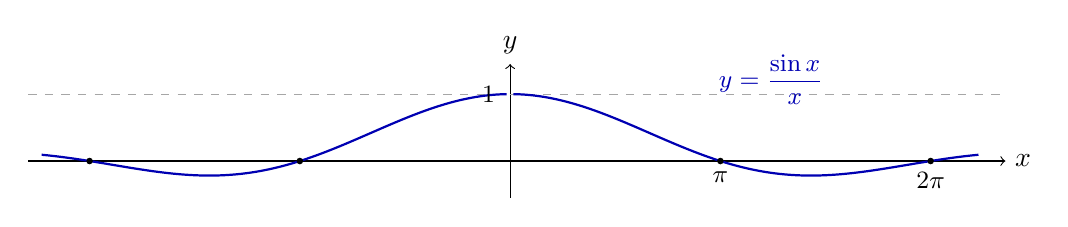
\begin{tikzpicture}[scale=0.85]
    % 坐标轴
    \draw[->] (-7.2,0) -- (7.4,0) node[right] {$x$};
    \draw[->] (0,-0.55) -- (0,1.45) node[above] {$y$};
    % 渐近水平线 y = 1
    \draw[dashed,gray!70] (-7.2,1) -- (7.4,1);
    % 曲线
    \draw[domain=0.05:7.0,samples=260,smooth,blue!70!black,thick]
      plot (\x,{sin(\x r)/\x});
    \draw[domain=-7.0:-0.05,samples=260,smooth,blue!70!black,thick]
      plot (\x,{sin(\x r)/\x});
    % 零点标记
    \foreach \k in {1,2} {
      \fill (\k*3.14159,0) circle (1.4pt);
      \fill (-\k*3.14159,0) circle (1.4pt);
    }
    % 标注
    \node[blue!70!black] at (3.9,1.22) {\small $y=\dfrac{\sin x}{x}$};
    \node[below] at (3.14159,-0.02) {\small $\pi$};
    \node[below] at (6.28318,-0.02) {\small $2\pi$};
    \node[left] at (-0.08,1) {\small $1$};
  \end{tikzpicture}
  \caption{$\sin x/x$ 的图像。零点位于 $x=n\pi$，与无穷乘积
           $\prod_{n\ge1}(1-z^{2}/n^{2})$ 的零点一致。}
  \label{fig:sinc}
\end{figure}

% =====================================================================
\section{三种路径的比较}
% =====================================================================

表 \ref{tab:compare} 从工具、严格性与可推广性三方面对比上述三种证明。

\begin{table}[H]
  \centering
  \small
  \caption{三种证明路径的比较}
  \label{tab:compare}
  \begin{tabular}{@{}>{\raggedright\arraybackslash}p{2.4cm}
                     >{\raggedright\arraybackslash}p{4.9cm}
                     >{\raggedright\arraybackslash}p{4.7cm}@{}}
    \toprule
    \textbf{路径} & \textbf{核心工具} & \textbf{局限} \\
    \midrule
    Fourier 级数
      & 三角函数系的正交性、Dirichlet 收敛定理
      & 需先建立级数的逐点收敛理论 \\
    \addlinespace
    双重积分
      & Tonelli 定理、一次线性替换、半角恒等式
      & 仅对 $\zeta(2)$ 这类低阶情形奏效 \\
    \addlinespace
    Euler 乘积
      & Weierstrass 分解、幂级数系数比较
      & 依赖整函数因子分解这一较重的工具 \\
    \bottomrule
  \end{tabular}
\end{table}

三者之中，双重积分的证明最为``初等''：它不涉及任何级数收敛性的精细讨论，
只用到了非负项级数可交换求和与积分这一基本事实。而 Euler 乘积的证明
最具启发性，因为它直接推广到了 $\zeta(2m)$ 的封闭形式 \eqref{eq:zeta2m}。

% =====================================================================
\section{余论：奇数处的 \texorpdfstring{$\zeta$}{zeta} 值}
% =====================================================================

由 \eqref{eq:zeta2m}，所有偶数处的值都是 $\pi$ 的有理倍数。自然要问：奇数处如何？

\begin{itemize}
  \item $\zeta(3)=1.2020569\ldots$（Apéry 常数）。Apéry 于 1978 年证明了它
        是无理数，但其与 $\pi$ 的代数关系至今未知。
  \item 对一般的奇数 $2m+1\ge 5$，$\zeta(2m+1)$ 的无理性仍是公开问题。
  \item 已知的结果仅有：奇数处的 $\zeta$ 值中至少有一个无理数
        （Ball--Rivoal, 2000），并且这样的无理值有无穷多个。
\end{itemize}

从这个角度看，$\zeta(2)=\pi^{2}/6$ 是一个``过于幸运''的例外：
它恰好落在 Euler 乘积能够完全处理的那一类里。

\vspace{1em}
\keybox{\textbf{Basel 问题}\quad
  $\displaystyle \sum_{n=1}^{\infty}\frac{1}{n^{2}}=\frac{\pi^{2}}{6}$}

\appendix
% =====================================================================
\section{附录：数值验证}
% =====================================================================

下表列出部分和 $S_{N}=\sum_{n=1}^{N}n^{-2}$ 与 $\pi^{2}/6$ 的差，
可见误差以 $1/N$ 的速度衰减（因 $S_N=\zeta(2)-1/N+O(N^{-2})$）。

\begin{table}[H]
  \centering
  \caption{部分和与极限值的比较}
  \begin{tabular}{@{}rrr@{}}
    \toprule
    $N$ & $S_{N}$ & $\pi^{2}/6-S_{N}$ \\
    \midrule
    $10$      & $1.5497677$ & $9.5166\times10^{-2}$ \\
    $10^{2}$  & $1.6349839$ & $9.9502\times10^{-3}$ \\
    $10^{3}$  & $1.6439346$ & $9.9950\times10^{-4}$ \\
    $10^{4}$  & $1.6448341$ & $9.9995\times10^{-5}$ \\
    $10^{5}$  & $1.6449241$ & $1.0000\times10^{-5}$ \\
    \bottomrule
  \end{tabular}
\end{table}

误差每扩大十倍样本量才缩小一个数量级，这解释了为何纯数值方法难以猜出精确值——
要得到 $10$ 位有效数字，需累加约 $10^{10}$ 项。

\end{document}
